\chapter{Experiments and Performance}
\label{chapter:experiments.performance}

This chapter describes the various tests run to evaluate Warlock's performance
and reliability. We then plot the test results and analyze the graphs.

\section{Evaluation Process}

The test setup consists of a cluster of servers hosted on Amazon \abbr{EC2}%
\sidenote[3]{Amazon Elastic Compute Cloud (EC2) is a computing platform that
  allows us to provision servers on demand as a web service. For details, 
  see \url{http://aws.amazon.com/ec2/}
}. We can test our system on different hardware configurations using the
different \term{instance} types provided. The configuration of the two
instances used in our tests are shown in \tableref{amazon.instances}

\begin{table}
  \begin{tabular}{|l|l|l|}
    \hline
    \multicolumn{3}{|c|}{Amazon Instances} \\
    \hline
    Type & Attribute & Value \\ \hline
    \multirow{3}{*}{\term{m1.large}} & CPU & 4 EC2 Compute Units \\
     & Memory &  7.5 GB \\
     & Platform & 64-bit \\ \hline
    \multirow{3}{*}{\term{c1.xlarge}} & CPU & 20 EC2 Compute Units \\
     & Memory &  7 GB \\
     & Platform & 64-bit \\ \hline
    \hline
  \end{tabular}
  \caption[Amazon Instance Types]{%
    Amazon instances used for testing.   
  }
  \label{table:amazon.instances}
\end{table}

The test cluster consists of 3, 5, or 7 servers running Warlock and 1 server
running Basho Bench \citep{basho.bench}. The different cluster configurations
tested are

\begin{enumerate}[A.]
  \item 3 \term{m1.large} servers
  \item 5 \term{m1.large} servers
  \item 7 \term{m1.large} servers
  \item 3 \term{c1.xlarge} servers
\end{enumerate}

We have created different tests to test the performance variations with
different parameters. We first test raw performance of the system with
different cluster configurations. Then we test the change in performance
of the system with change in input parameters while keeping the cluster
static. Specifically, the tests are

\begin{enumerate}[1.]
  \item Write only requests only to master node
  \item Read only requests only to master node
  \item Write only requests to all nodes
  \item Read only requests to all nodes
  \item Mixed requests to cluster
  \item Variation in number of concurrent client connections
  \item Variation in read to write ratio
  \item Variation in payload size
  \item Different back ends
  \item Change in location of the bench client
\end{enumerate}

We also measure the system health in terms of CPU usage, memory usage and
process count providing an idea about the resource consumption.

%\section{Load Testing}

%\section{Failure Testing}

%safety testing, liveliness testing

%bugs, fixes, master election

%integration with kingdom backend

%\todo{evaluation of running the code in production,
%live on test, staging, 20\% of production etc.}

%\todo{Add tables for results?}

\section{Results}

\subsection{General Performance}

\begin{figure}
  \begin{whole}
    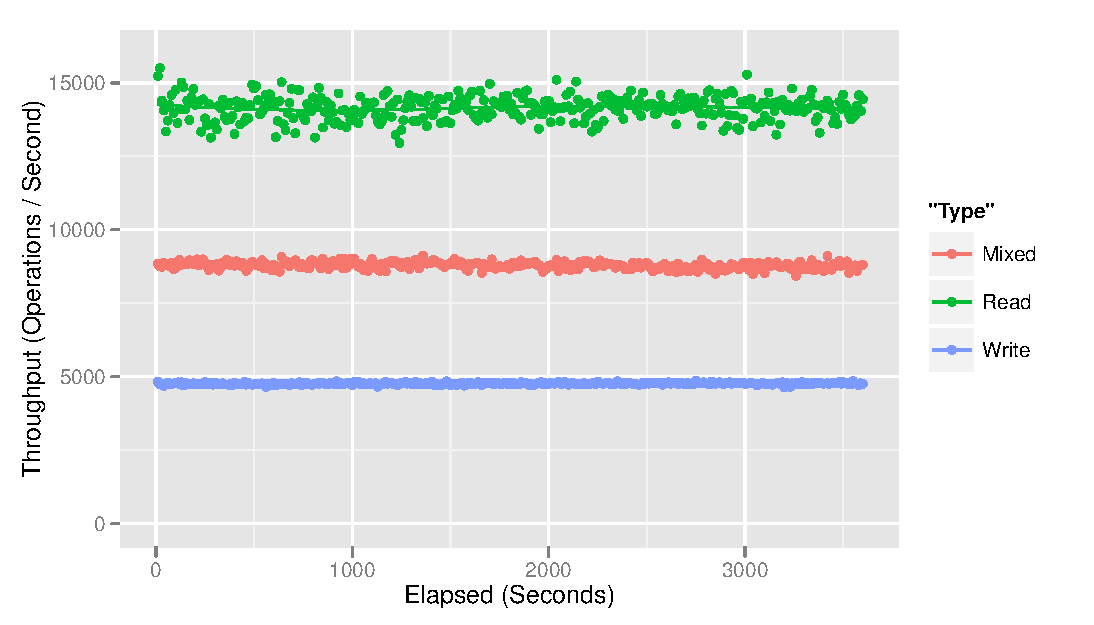
\includegraphics[width=\wholewidth]{d3-d4-d5-summary}
    \caption[General Performance Throughput Test]{%
      A simple performance test to evaluate throughput with different request
    types.}
    \label{figure:res.general.performance}
  \end{whole}
\end{figure}

\figureref{res.general.performance} shows the performance of Warlock based on
type of requests when run for an hour. All the server were of \term{c1.xlarge}
type. The requests were generated by a single bench servers with 10 concurrent
connections and handled by a 3 node Warlock cluster. The mixed requests 
consisted of ${}^2/_3$ read , ${}^1/_6$ write and ${}^1/_6$ delete requests.

The results show that the Warlock can handle $\approx$ 5,000 writes/second, 
$\approx$ 14,000 reads/second and $\approx$ 8,000 mixed requests/second. The
performance remains consistent throughout the test. This also helps us
acknowledge that Warlock can handle the load generate in Magic Land.

\begin{figure}
  \begin{whole}
    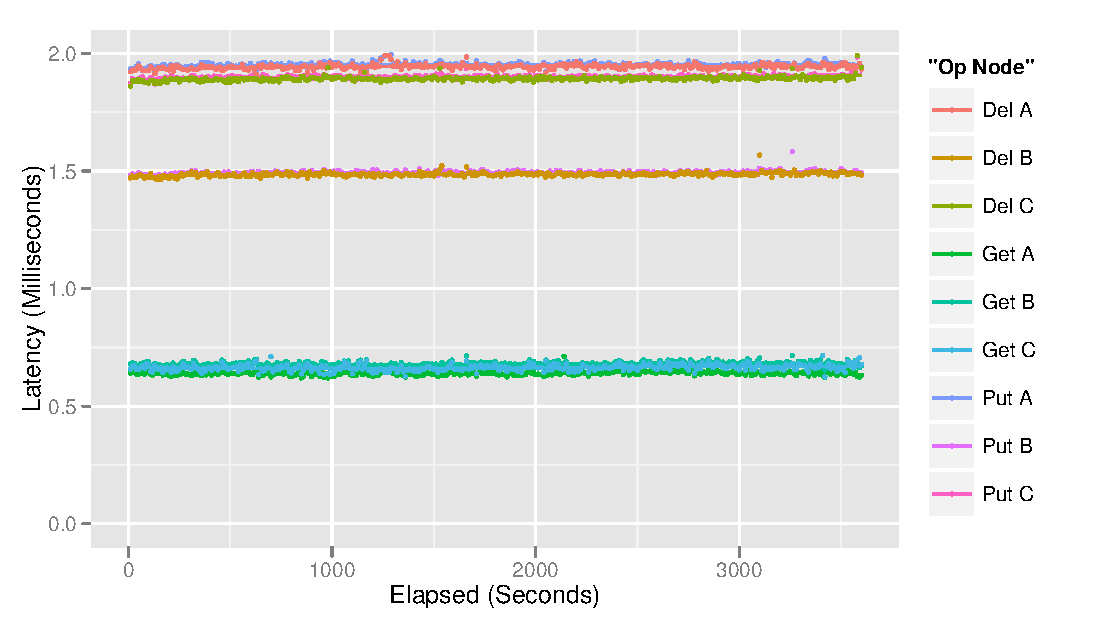
\includegraphics[width=\wholewidth]{d5-latencies}
    \caption[General Performance Latency Test]{%
      Performance test that shows us the change in latency based on the request
      types.
    }
    \label{figure:res.general.latency}
  \end{whole}
\end{figure}

\figureref{res.general.latency} shows us the change in request latency%
\sidenote{
  \emph{Latency}: The total time taken to issue a request, process it and
  receive a response from the client's perspective.
} with change in request types. We observe that the \term{GET} requests have the
lowest latency. This is expected since these requests do not have to go through
the protocol. The \term{PUT} and \term{DEL} requests are close together since
they are very much similar. We also observe that \term{PUT} and \term{DEL} 
requests sent to the master have lower latency as expected since we save a
message trip.

\subsection{Read to Write Ratio}

\begin{figure}
  \begin{whole}
    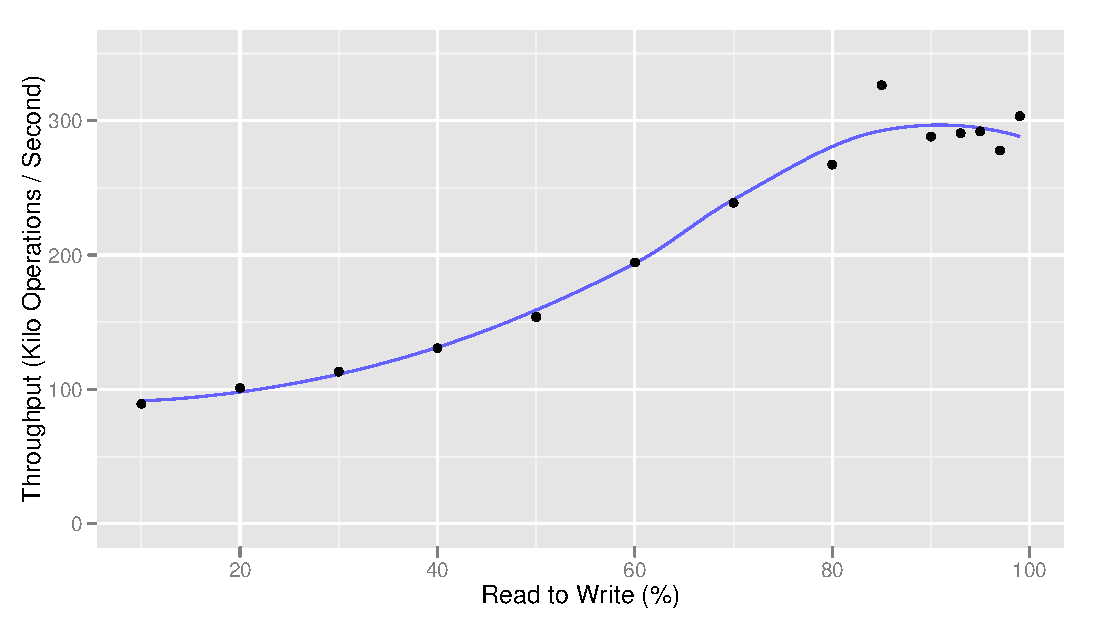
\includegraphics[width=\wholewidth]{read-ratio-variance}
    \caption[Read to Write Ratio Test]{%
      Test depicting the variation of performance with increase in read
      to write ratio.
    }
    \label{figure:res.read.write.ratio}
  \end{whole}
\end{figure}

We observe that the performance of the system increase with the increase in
the read to write ratio, as shown in \figureref{res.read.write.ratio}. This is
expected since the system is tuned to handle more number of reads than writes.

The test was run with a single bench server with 100 concurrent connections to
a 3 node Warlock cluster.

\subsection{Concurrency}

\begin{figure}
  \begin{whole}
    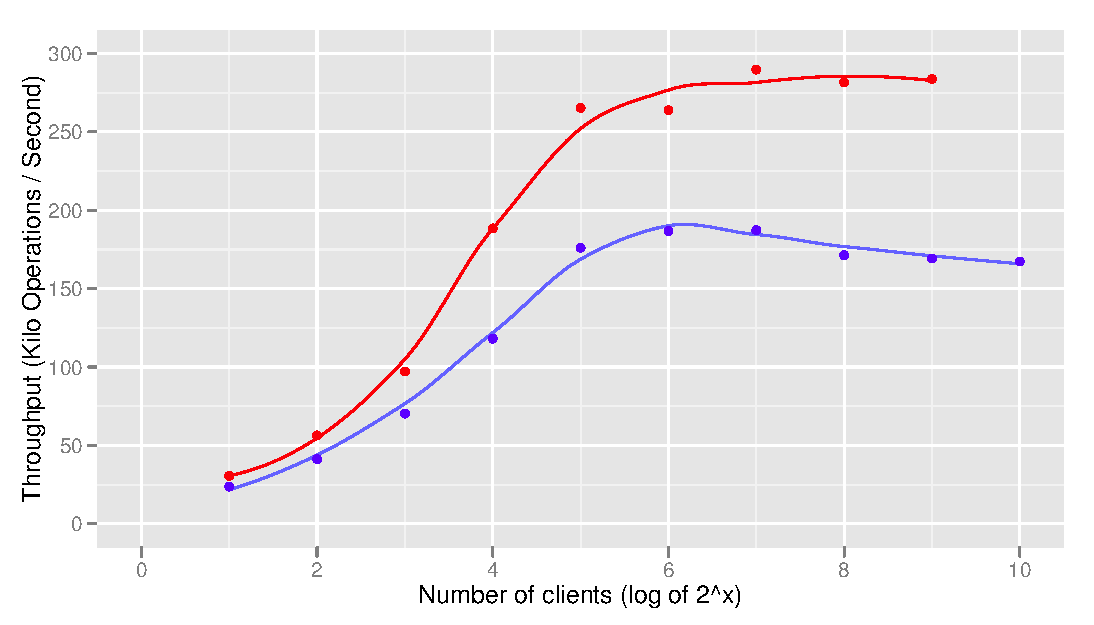
\includegraphics[width=\wholewidth]{concurrency-variance}
    \caption[Concurrency Test]{%
      Test shows the performance variation of the system with exponential
      increase in number of client connections.
    }
    \label{figure:res.concurrency}
  \end{whole}
\end{figure}

We can connect to a Warlock cluster in two ways \dash{} RPC and Redis protocol
as discussed in \sectionref{a.n.d.client.conn}. The \textcolor{red}{red} line
in \figureref{res.concurrency} indicates the successful requests using the
Redis protocol and the \textcolor{blue}{blue} line indicates those using RPC.

We observe that the throughput increases upto 64 concurrent connections and
stays constant after that. Warlock cluster timed out on some requests when
using RPC with 1024 connections. Also, we were unable to test the Redis protocol
with concurrency level of 1024 due to Basho Bench becoming unresponsive.

The distribution of read and write requests for this test was ${}^4/_5$ and
${}^1/_5$ respectively.

\subsection{Payload Size}

\begin{figure}
  \begin{whole}
    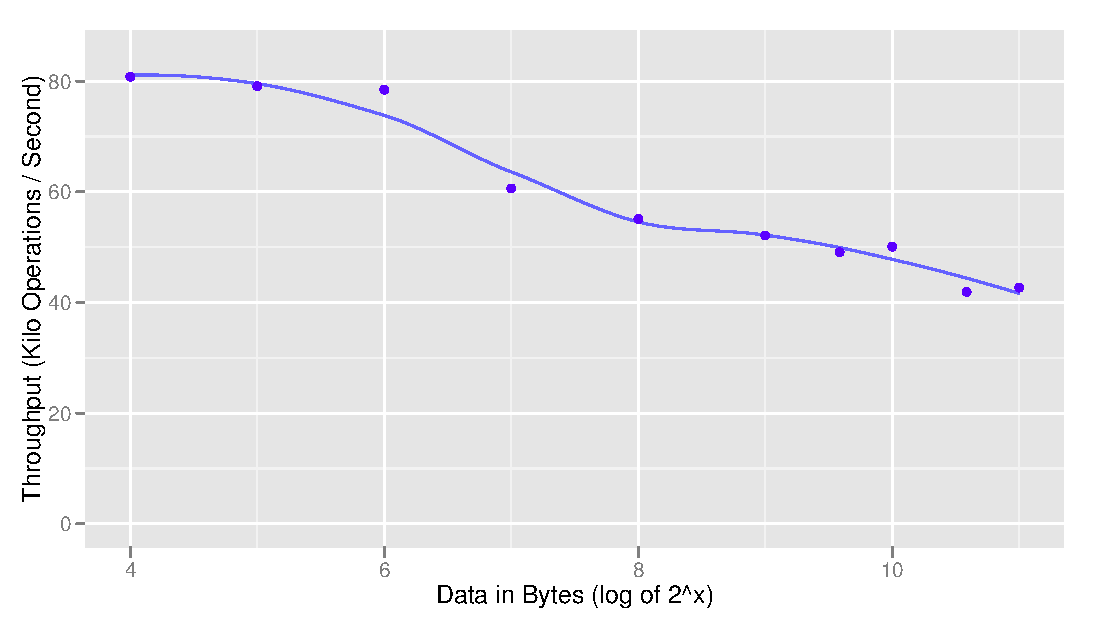
\includegraphics[width=\wholewidth]{payload-variance}
    \caption[Payload Throughput Test]{%
      Test indicates the variation of system throughput with exponential
      increase in message size.
    }
    \label{figure:res.payload.throughput}
  \end{whole}
\end{figure}

\figureref{res.payload.throughput} shows us the change in system throughput
with increase in payload size. We observe a near linear decrease in performance
which is expected since the algorithm is $O(n)$, where $n$ is the number of
messages.

\begin{figure}
  \begin{whole}
    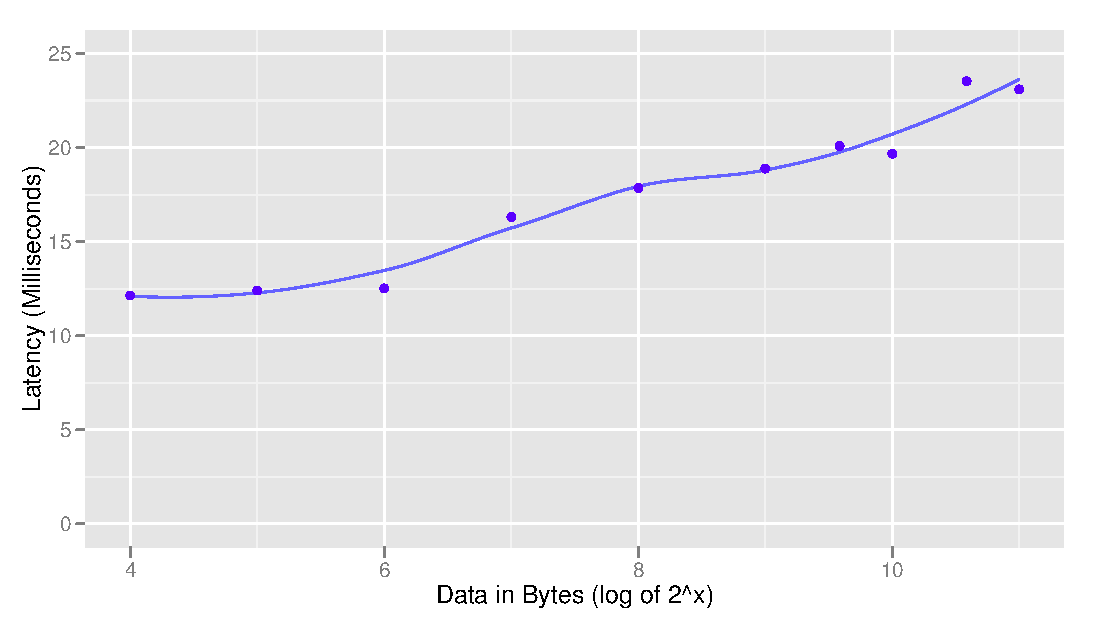
\includegraphics[width=\wholewidth]{latency-variance}
    \caption[Payload Latency Test]{%
      Test depicts the change in latency with exponential increase in payload
      size.
    }
    \label{figure:res.payload.latency}
  \end{whole}
\end{figure}

\figureref{res.payload.latency} shows the latency result for the same test. We
again observe a nearly linear increase in latency.

The amount of read and write requests for this test was ${}^4/_5$ and
${}^1/_5$ of the total respectively.


